\documentclass[12pt, a4paper]{article}
\usepackage[utf8]{inputenc} 
\usepackage[english]{babel}
\usepackage{latexsym}
\usepackage{url}
\usepackage{fancyhdr}
\usepackage{hyperref}
\usepackage{xparse}
\usepackage{graphicx}
\usepackage{amssymb}
\usepackage{multirow}
\usepackage{pmboxdraw}


\usepackage{mathtools}

\DeclarePairedDelimiter\ceil{\lceil}{\rceil}
\DeclarePairedDelimiter\floor{\lfloor}{\rfloor}


\title{SAD calculation of two monochrome images}
\author{Francesco Urbani}
\date{\today}



\frenchspacing
\pagestyle{fancy}
\fancyhf{}
\rhead{\bfseries\thepage}


\renewcommand{\sectionmark}[1]{\markboth{\thesection.\ #1}{}}



\begin{document}
\maketitle
\newpage
\tableofcontents
\newpage 
\listoffigures
\newpage

\section{Project specifications}


Design a synchronous digital system that calculates the SAD value, defined as the sum of the magnitude of the differences of each pixel of two monochrome images, image A and image B. Each pixel's value is stored in \texttt{N}-bits and each images has \texttt{px} pixels per side.
The circuit has a clock, a reset and an enable signals as input together with the signals PA and PB representing one pixel of each image getting into the system from the outside, sequentially.
The circuit has a \texttt{M}-bits output signal called SAD, where:

\begin{equation}
    2^\texttt{M} \ge (2^\texttt{N}-1) \cdot \mbox{\texttt{px}}^2
\end{equation}

and a DATA\_VALID signal which is set when the SAD calculation is completed.

When the reset is active, SAD and DATA\_VALID go to 0. If the enable signal is zero the system does not change its state.



\section{Algorithm description}
In order to meet the specification's constraints, I've designed -- using the hardware description language VHDL -- a synchronous digital circuit, that takes as input two monochrome images modeled as two N-bits signals and it outputs the value of the SAD once the calculation was over.

The signals representing the images enters into two PIPO registers whose output is then subtracted and made positive. 

The output of the subtraction is then fed into a M-bits phase accumulator which increases its value at every clock cycle.

The output of the phase accumulator represents the value of the \textit{current} SAD.


\section{Architecture}

The architecture chosen is the following:



\begin{figure}
\centering
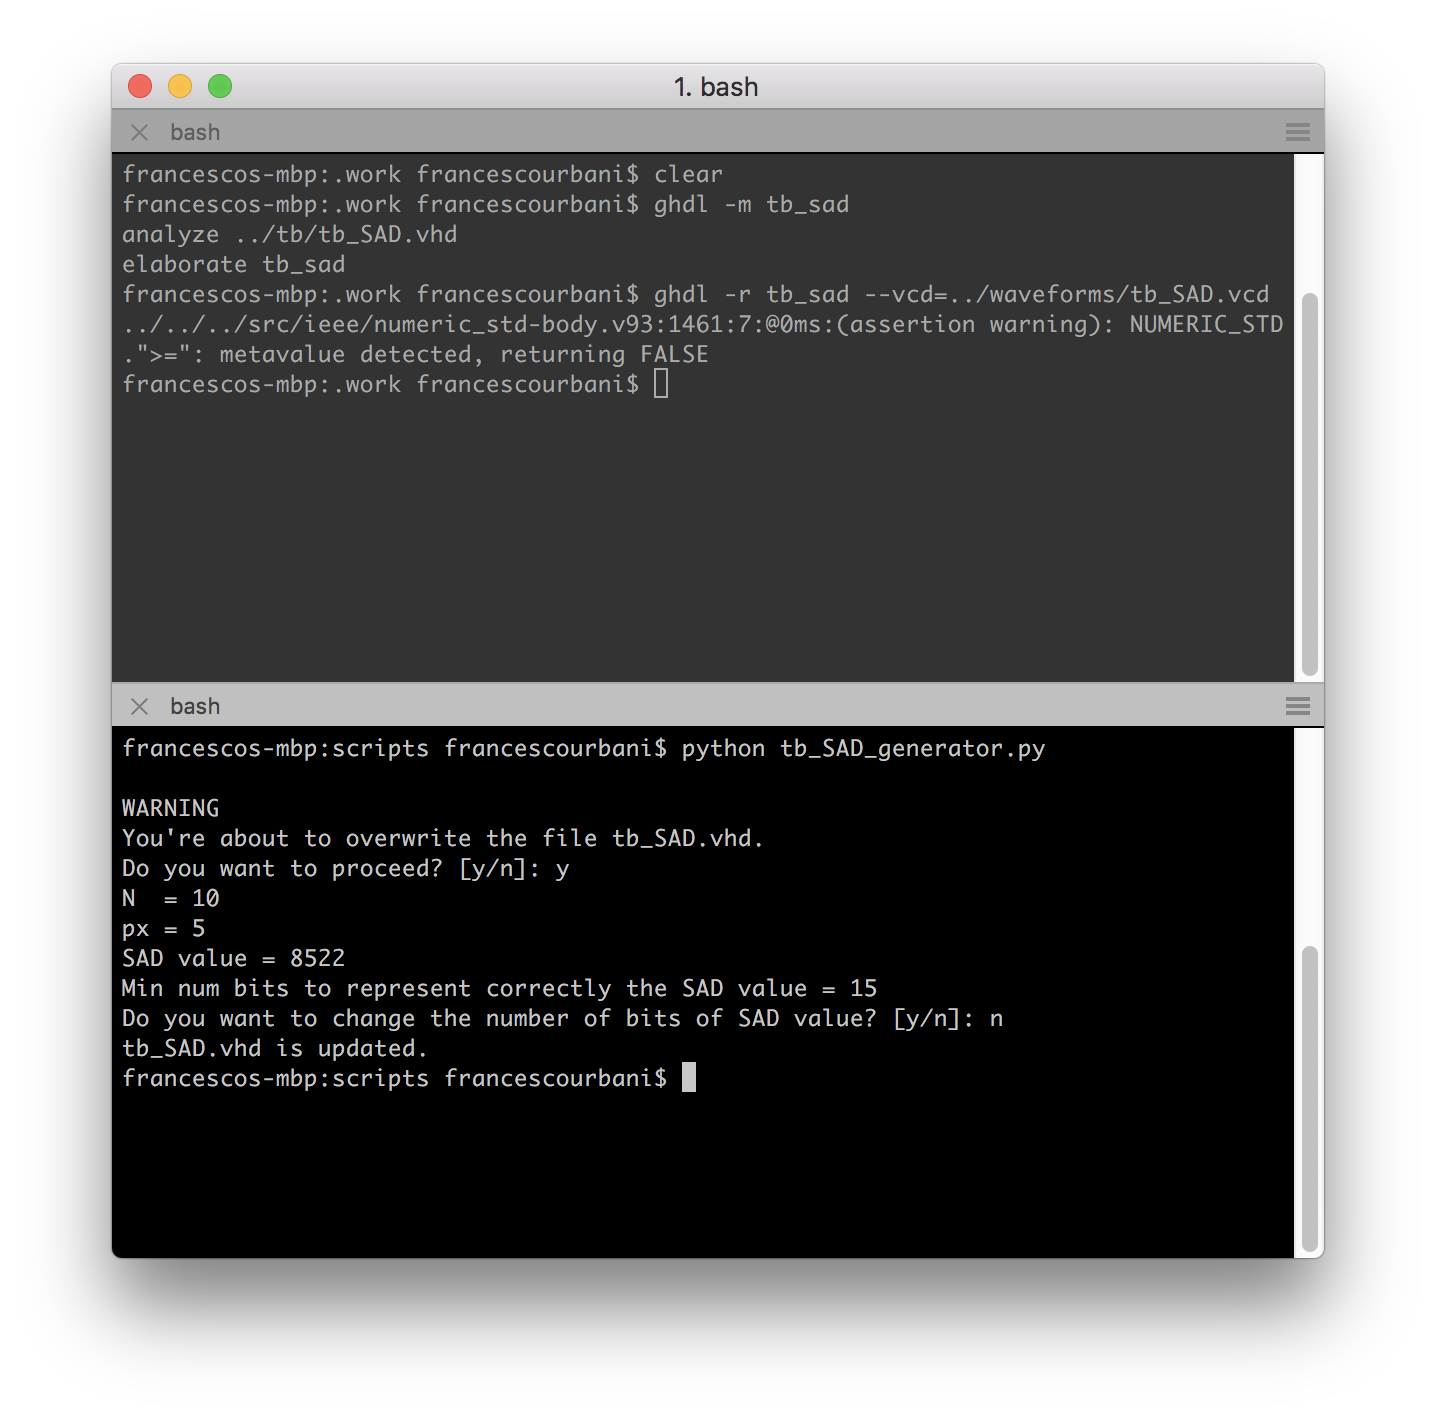
\includegraphics[scale=0.5]{../screenshots/fig1.png}
\caption{SAD architecture}\label{fig:7}
\end{figure}




The images are fed into the system by means of two signals, called PA and PB, whose size is N, i.e. the number of bits representing the pixel grade on a scale from 0 (i.e. 100\% black) to $2^N-1$, typically 255 (i.e. 100\% white).

Being the system synchronous, it works on the rising-edge clock.

The other two inputs are the reset (active high) and the enable, that prevents the SAD value to be updated when it's low.

The two outputs are SAD and DATA\_VALID. 

SAD represent the actual information we are interested in, and it's defined as the sum of the absolute differences of each pixel of the two images. 
Therefore it's value is updated at each clock cycle and its only freezed when the enable is low or the calculation is completed.

DATA\_VALID goes high when the SAD calculation is completed and stays high until the system is reset.




\section{VHDL}

A structural approach has been followed.
After writing the \texttt{.vhd} files describing all the components that I would have been using in the top-level component, I've simply wired them up together to create the final design.
The only two components described with a \textit{behavioral} approach have been \texttt{counter.vhd} and \texttt{subtractor.vhd}.



\subsection{Test benches}



In order to create a relevant test bench for \texttt{SAD.vhd} that would replicate an actual real-life situation, which means two images where every pixel is different to the adjacent pixel, a Python script has been developed.
\newline

The script (see \texttt{./scripts/tb\_SAD\_generator.py}) takes as input the number of bits representing each pixel value (\texttt{N}) and the number of pixels/side, i.e. the square root of the total number of pixels composing each image (\texttt{px}).
It also calculates the minimum number of bits necessary to store the SAD value without loosing information which is:
\begin{equation}
    \ceil[\big]{\ \log_2( (2^\texttt{N}-1) \cdot \texttt{px}^2 )\ } 
\end{equation}
and asks the user whether he wants to increase it.
\newline

After that the script generates two square matrices with integer elements in the range $[0, 2^N)$, calculates a third matrix whose elements are the magnitude of the difference of the former two matrices' elements and eventually calculates the overall sum of it's elements, i.e. the expected SAD value.
\newline


Afterwards it generates the test bench file \texttt{tb\_SAD.vhd} adherent to the model so that comparing the model to the waveform result would be straightforward.

\newpage
\subsection{Compiling instructions}

I've used the open-source compiler \href{http://ghdl.free.fr/}{GHDL} to compile the VHDL code in conjunction with the waveform viewer \href{http://www.logicpoet.com/scansion/}{Scansion} which is a nice alternative to \href{http://gtkwave.sourceforge.net/}{GTKWave} for macOS.
\newline

Once organized the folder like this:

\begin{verbatim}
.
├── .work
├── scripts
├── src
├── tb
├── vivado
└── waveforms
\end{verbatim}

move into \texttt{.work/} and from your terminal type:
\newline

\texttt{ghdl -i ../src/*}

\texttt{ghdl -i ../tb/*}
\newline

to import all the \texttt{.vhd} files into the working directory. Then:
\newline

\texttt{ghdl -m sad}
\newline

to compile the top-level component. That will compile all the components 
instantiated into the top-level component as well. Then type:
\newline

\texttt{ghdl -m tb\_sad}
\newline

to compile the test bench of the top-level component. And finally:
\newline

\texttt{ghdl -r tb\_sad --vcd=../waveforms/tb\_SAD.vcd}
\newline

to create the waveform file \texttt{tb\_SAD.vcd} which can be afterwards opened with one of those two above mentioned waveform viewers.






\section{Vivado}









\end{document}